% ---------------------------------
% -- Assignment 1: Chapter 1, #1 --
% -- Math 4171 --------------------

% Set document type
\documentclass[11pt,oneside]{extarticle}


\usepackage{amsmath}
\usepackage{amssymb}
\usepackage{amsthm}
%\usepackage{thmtools}
\usepackage{fontspec}
\usepackage[margin=0.5in]{geometry}
\usepackage{inputenc}
\usepackage{setspace}
\usepackage{fancyhdr}
\usepackage{garamondx}
\usepackage{graphicx}
\usepackage{hyperref}
\usepackage{float}
\usepackage{listings}
\usepackage{newtxmath}
\usepackage{solarized-light}
\usepackage{xcolor}
%\usepackage{lmodern}

\usepackage[default]{sourcecodepro}
\usepackage[T1]{fontenc}
%\usepackage{inconsolata}
% Real number symbol
\newcommand{\Real}{\mathbb{R}}

% Set typewriter font to Source Code Pro
\renewcommand{\ttfamily}{\tiny\sourcecodepro}

% Change enumerator to use letters i.e., a, b, c, ...
\renewcommand{\theenumi}{\alph{enumi}}

\setlength{\belowcaptionskip}{-12pt}
%\setttfont{

\begin{document}
\section{Chapter 3}

\subsection{Exercise 1}

The \textsc{Rosenbrock} function

$$
f:\Real^2 \rightarrow \Real, x \mapsto 100(x_2-x_1^2)^2 + (1-x_1)^2,
$$

also compare \url{http://en.wikipedia.org/wiki/Rosenbrock_function}, is frequently
utilized to test optimization methods.

\begin{enumerate}

    \item The absolute minimum of $f$, at the points $(1,1)^T$, can be seen 
        without any calculations. Show that it is the only extremal point.

    All local (and thus global) extrema occur at critical points of $f$, therefore
    it is sufficient to show that the only critical point exists at $(1,1)^T$.

    $$\nabla f(x)=\begin{pmatrix}
        200(x_2 - x_x^2 ) (-2x_1) - 2(1-x_1) \\
        200(x_2-x_1^2) \\
    \end{pmatrix}$$

    The only solution to $\nabla f(x) = 0$ is $x=(1,1)^T$, which is at the
    absolute minimum $(1,1)^T$, which we already have. There are no other critical
    points, therefore this is the only extrema.

    \item Graph the function $f$ on $[-1.5,1.5]\times [-0.5,2]$ as a 3D plot or
        as a level curve plot to understand why $f$ is referred to as the
        \emph{banana function} and the like.

        \begin{figure}[H]
            \caption{The \textsc{Rosenbrock} Function}
        \label{fig:rosenbrock}
        \begin{center}
            %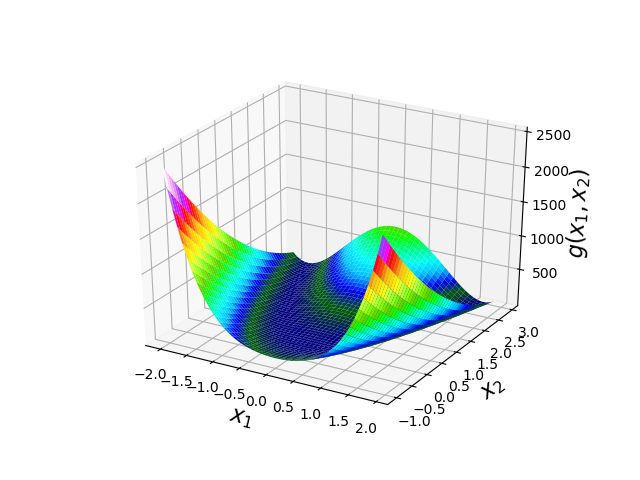
\includegraphics[scale=0.8]{/home/jacques/repos/math4171/assignment1/figures/fig1-1.png}
            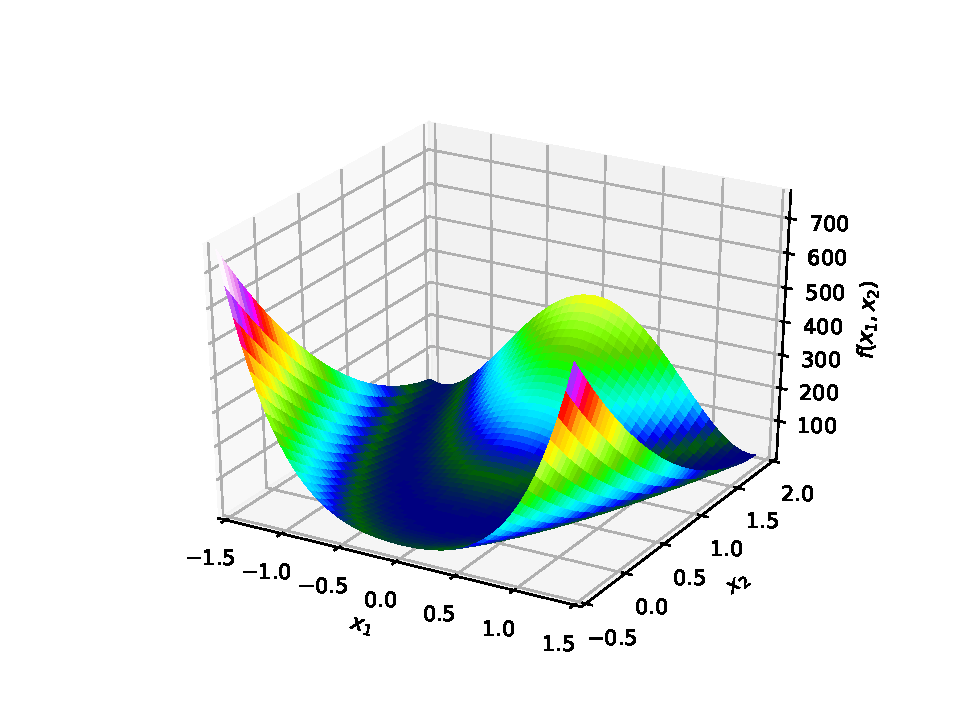
\includegraphics[scale=0.8]{./figures/fig1-1.pdf}
        \end{center}
    \end{figure}

    \item Implement the \textsc{Nelder-Mead} method. Visualize the level curves of the
        given function together with the polytope for each iteration. Finally
        visualize the trajectory of the centres of gravity of the polytopes!

    \begin{figure}[H]
            \caption{Convergence of polytopes to solution}
        \label{fig:contours}
        \begin{center}
            %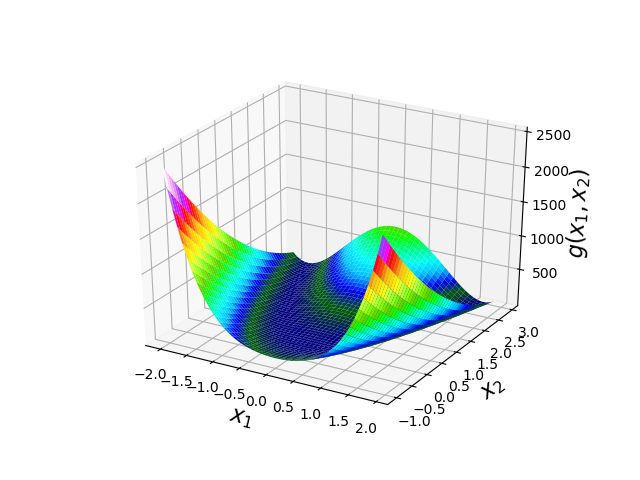
\includegraphics[scale=0.8]{/home/jacques/repos/math4171/assignment1/figures/fig1-1.png}
            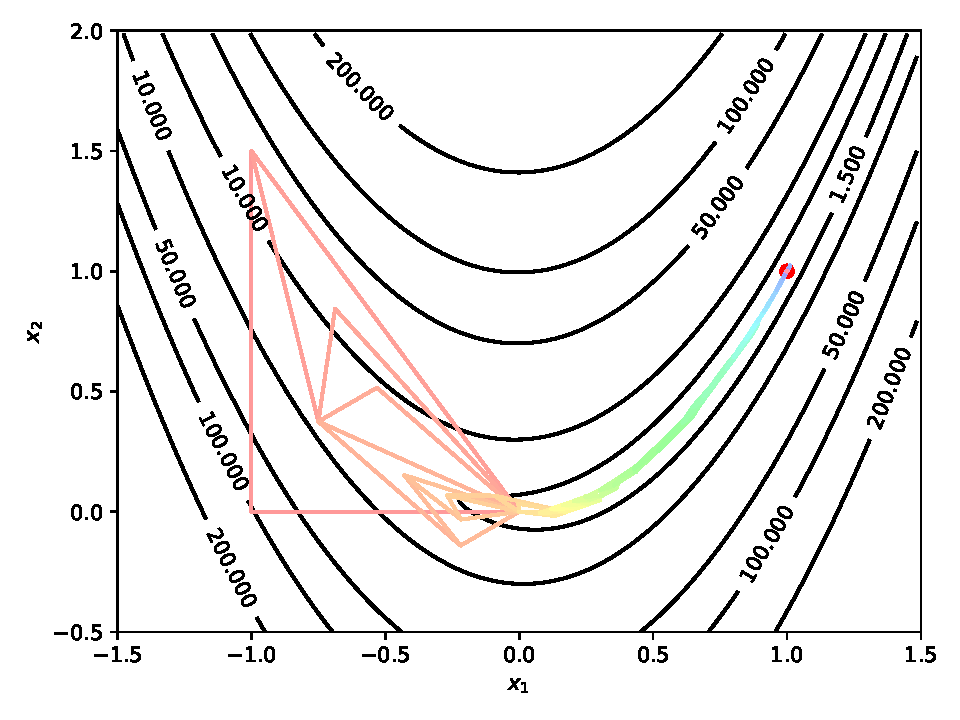
\includegraphics[scale=0.8]{./figures/fig1-2.pdf}
        \end{center}
    \end{figure}
    
    \begin{figure}[H]
            \caption{Convergence of polytopes to solution}
        \label{fig:contours}
        \begin{center}
            %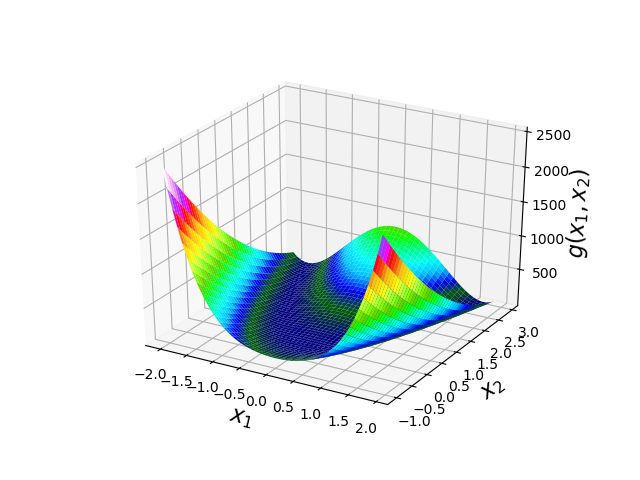
\includegraphics[scale=0.8]{/home/jacques/repos/math4171/assignment1/figures/fig1-1.png}
            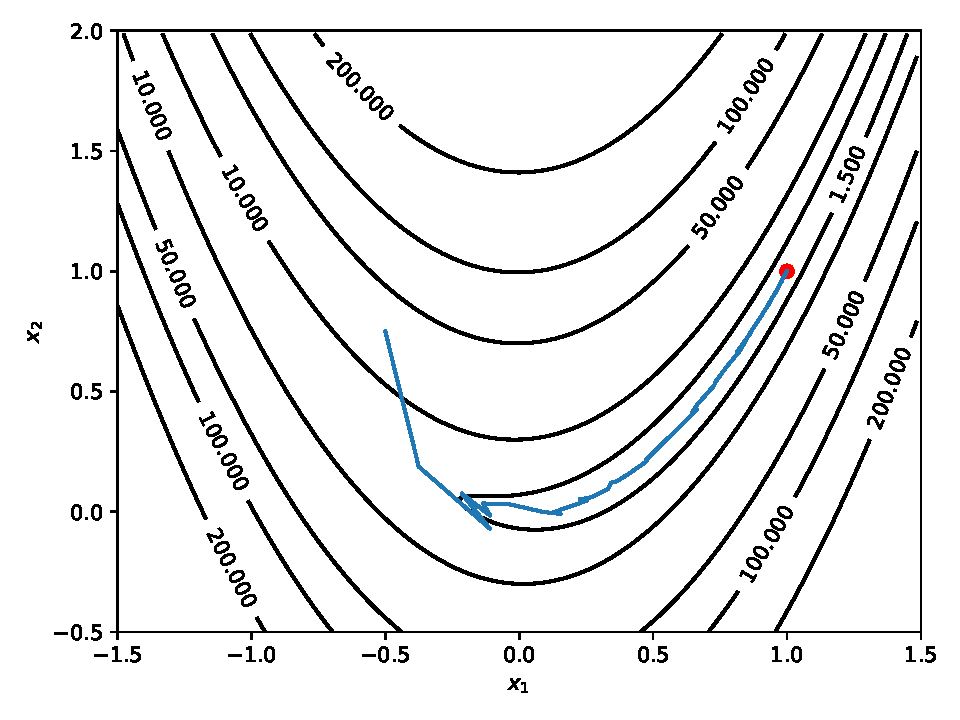
\includegraphics[scale=0.8]{./figures/fig1-3.pdf}
        \end{center}
    \end{figure}

    \item Test the program with the starting polytope given by the vertices
        $(-1,1)^T$, $(0,1)^T$, $(-0.5,2)^T$ and the parameters
        $(\alpha,\beta,\gamma):=(1,2,0.5)$ and $\varepsilon := 10^{-4}$ using
        the \textsc{Rosenbrock} function. How many iterations are needed? What
        is the distance between the calculated solution and the exact minimizer
        $(1,1)^T$?

    \item Find $(\alpha, \beta, \gamma ) \in \left[ 0.9,1.1\right] \times
        \left[1.9,2.1\right] \times \left[0.4,0.6\right]$ such that with
        $\varepsilon := 10^{-4}$ the algorithm terminates after as few iterations
        as possible. What is the distance between the solution and the minimizer
        $(1,1)^T$ in this case?

    \item If the distance in \emph{e} was greater than in \emph{d}, reduce
        $\varepsilon$ until the algorithm gives a result---with the $(\alpha,\beta,\gamma)$,
        found in \emph{e}---which is not farther away from $(1,1)^T$ and at the same
        time needs fewer iterations than the solution in \emph{d}.

\end{enumerate}

\section{Appendix I}

\begingroup
\fontseries{t}\selectfont
\lstinputlisting[language=c++]
{../src/arcmath/MinNelderMead.hpp}
\endgroup

\begingroup
\fontseries{t}\selectfont
\lstset{language=c++,
    showstringspaces=false
    %basicstyle=\roboto\scriptsize,
    %keywordstyle=\color{blue}\roboto,
    %stringstyle=\color{red}\roboto,
    %commentstyle=\color{green}\roboto
    %morecomment=[1]\color{magenta}]{\#}
}
\lstinputlisting[language=c++]
{../src/arcmath/MinNelderMead.cpp}
\endgroup
%\begin{lstlisting}
%for( int i = 0; i < n; i++ ){
    %do something
%}
%\end{lstlisting}



\end{document}
